%
%  $Description: Survey on Orchestration$
%

\documentclass[10pt,twocolumn]{article}
\usepackage{times,mathptmx,fullpage}
% Allows you to put literal text into your document without having LaTeX try to interpret it.
\usepackage{verbatim}
% Sorts citations numerically and "combines" adjacent ones
\usepackage{cite}
% Allows you to individually label subfigures in a multi-part figure
\usepackage{subfigure}
% Allows the definition of macros that are smart about adding space after text in a macro
\usepackage{xspace}
% To use external images
\usepackage{graphicx}

% Redefine the percentage of the page that can be used for floats (figures, tables, etc.)
\renewcommand\floatpagefraction{.9}
\renewcommand\dblfloatpagefraction{.9}
\renewcommand\topfraction{.9}
\renewcommand\dbltopfraction{.9}
\renewcommand\bottomfraction{.9}
\renewcommand\textfraction{.1}
\setcounter{totalnumber}{10}
\setcounter{topnumber}{10}
\setcounter{dbltopnumber}{10}
\setcounter{bottomnumber}{10}

% Set values for float separation from text
\setlength{\floatsep}{1.5ex plus1.0ex minus 0.2ex}
\setlength{\dblfloatsep}{1.5ex plus1.0ex minus 0.2ex}
\setlength{\textfloatsep}{1.5ex plus1.0ex minus 0.2ex}
\setlength{\dbltextfloatsep}{1.5ex plus1.0ex minus 0.2ex}
\setlength{\abovecaptionskip}{0.5ex}
\setlength{\belowcaptionskip}{0.5ex}

% Don't allow widows or clubs - single lines at the start/end of a column
\widowpenalty=10000
\clubpenalty=10000

\newcommand{\latex}{\LaTeX\xspace}
\pagestyle{plain}

%-------------------------------------------------------------------------
\begin{document}

\title{A Survey on Virtual Machine and Container Orchestration}

\author{
Aneesh Neelam \\
\textit{Univ. of California, Santa Cruz} \\
\textit{aneelam@ucsc.edu}
}

\maketitle
\thispagestyle{empty}

\begin{abstract}

  Data center administrators and site-reliability engineers create virtual machines or containers to run their applications, with desired redundancy requirements and automated coordination between the replicas.
  This is called the orchestration of the various computing, storage and network resources of the data center.
  To automate the orchestration process, different tools have been developed in the past couple of decades.
  Each tool was designed differently, with different intents and priorities but they also have a lot in common.
  This survey is on the various orchestration tools available to data center administrators, site reliability engineers and software engineers;
  and aims to be a comprehensive guide that helps data center administrators in choosing the cloud platform and the orchestration tool.

\end{abstract}

%-------------------------------------------------------------------------
\section{Introduction}

With the advent and proliferation of virtualization, computing as a service has taken off.
Now there are multiple cloud service providers such as Google Cloud, Amazon Web Service, Microsoft Azure, etc.
The operators of these cloud services typically have their own data centers, each consisting of thousands of physical machines connected via a high speed and very low latency network such as Infiniband (IB) ~\cite{intro_infiniband}.
Data center operators use various tools to automate the process of management, provisioning and scaling the resources for their customers.

Orchestration tools have been developed to ease the operation of a data center.
Tools such as OpenStack's Heat have been used to manage Linux kernel virtual machines ~\cite{openstack}.
There are many other such tools such as Chef and Ansible for virtual machines ~\cite{chef, ansible}.
Container Orchestration tools such as Docker Swarm, Kubernetes, Mesos have been developed to manage containers on mostly Linux machines ~\cite{docker_swarm, kubernetes, mesos}.
In this survey however, we shall focus more on orchestration of containers than virtual machines.

Using these orchestration tools, data center operators can boot up virtual machines or containers on the physical machines, and control the entire the data center as a single entity, provision the necessary resources, and deploy and managing applications.
These orchestration tools can also be used to automate replication of processes, fault tolerance, failure detection and recovery, live migration of processes or entire virtual machines between physical machines, and also set up coordination between the processes to make the development of applications for the distributed system easier ~\cite{live_migration, xen}.
Some orchestration tools also enforce quotas for processes, ensure that Service-level agreements are adhered to and can also be used to keep track of the overall resource utilization and power consumption of the data center.

In this survey, the performance of these orchestration tools shall be compared.
Also, these orchestration tools may also have different guarantees of tolerance when there is a failure or network partition.
According to the CAP theorem, only two out of three: presence of network partitions, availability and consistency can be guaranteed by any distributed system ~\cite{CAP_theorem}.
In which case, there may be different methods the orchestration tools employ for error recovery and maintain high reliability, offering various combinations of two out of the three things for applications to easily support.

In the next section, we shall see some of the past work on virtualization, the use of virtual machines and containers, and the approaches taken by the different virtualization technologies to enforce isolation between applications.
In Section 3, we shall describe how virtual machines and containers controlled by the various orchestration tools.
In Section 4, we analyze the limitations, evaluate the performance and ease of use, and also compare the different approaches they take for coordination and failure.
We then discuss possible future work in the field in Section 5, and we then conclude in Section 6.

\begin{figure*}
\centering
  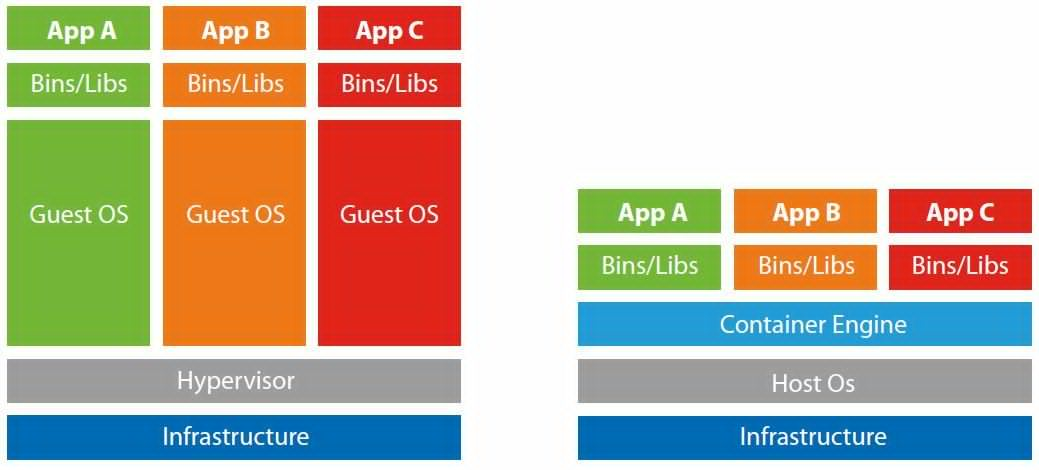
\includegraphics[width=\textwidth]{container-vs-vm.jpg}
    \caption{Differences between Virtual Machines and Containers~\cite{intro_containerisation}
      \label{overflow}}
\end{figure*}

%-------------------------------------------------------------------------
\section{Background}

The increasing proliferation and popularity of virtualization technology were necessary for the data center, and cloud service providers to thrive.
Virtual machines allowed for running more isolated virtual operating systems or applications on lesser number of physical machines.
The use of these virtual machines could be leased out to third-parties, providing a revenue stream for people who may have powerful physical machines but are unable to push them to their full potential.
Consequently, cloud computing has made the concept of computing as a utility possible ~\cite{berkeley_cloud}.
Virtualization, in this context, is the task of creating virtual hardware and running actual operating systems and applications on top of them.
Each of these virtual machines is isolated and independent from one another and are managed by a hypervisor that is running on the physical hardware or on the host operating system ~\cite{xen}.

Virtualization technology is now decades old, with every major operating system that runs on servers having inbuilt virtualization support without the need for a third-party hypervisor.
For example, the Linux kernel has KVM and Microsoft Windows Server has Hyper-V.
Both also have well-documented endpoints for various front-ends to interface with, providing data center operators and server administrators with many tools to automate and manage their machines.

A similar development is going on with containers on these operating systems as well. Like Cgroups in the Linux kernel, Hypervisor.framework in Apple macOS and Hyper-V in Microsoft Windows.
Container enngines that provide a cross-platform frontend but make use of the respective container support structure in the host operating system have been developed, of which the most prominent is Docker ~\cite{intro_docker}.

Virtual machines are a complete hardware virtualization, and there is a full-fledged guest operating system on which applications are run. Virtual machines enable the use of legacy applications that require legacy operating systems that only run on legacy hardware.
The necessary legacy hardware can be emulated by the hypervisor, allowing the unmodified operating systems and applications to be run.
There is also paravirtualization where a significant ioncrese of performance can be achieved with some changes to the guest operating system, but it still does not entail modifying the application.

However, containers provide the isolation of virtual machines without much of the overhead. There is no guest operating system, and the host kernel itself enforces isolation ~\cite{intro_containerisation}.
However, that would also mean that the applications would have to be able to execute directly on the host operating system.
Hence, this technique may not be used to run legacy applications.

Figure 1 shows the differences between virtual machines and containers ~\cite{intro_containerisation}.
Containers, with none of the overhead of virtual machines and the lack of guest operating systems, can be used to start up many orders of magnitude number of applications on the same host kernel.
Containers are still new, however, and the implementation in the various operating system kernels may have bugs that compromise this isolation.

Orchestration tools for managing virtual machines and containers on many physical machines in a cluster have been developed.
Tools for virtual machines that we shall evaluate in this survey include OpenStack ~\cite{openstack}, Chef ~\cite{chef} and Ansible ~\cite{ansible}.
Some of the tools for containers we shall cover in this survey are Docker Swarm ~\cite{docker_swarm}, Kubernetes ~\cite{kubernetes}, Mesos ~\cite{mesos}.

%-------------------------------------------------------------------------
\section{General Comparison}



\subsection{Virtual Machine Orchestration}



\subsection{Container Orchestration}



%-------------------------------------------------------------------------
\section{Evaluations}



\subsection{Performance}



\subsection{Ease of Use}



\subsection{Protocols used}



\subsection{Use Cases}



\subsection{Caveats}




%-------------------------------------------------------------------------
\section{Future of Orchestration}



\subsection{Use of Virtual Machines}



\subsection{Further Innovation and Development}



%-------------------------------------------------------------------------
\section{Conclusion}



%-------------------------------------------------------------------------
\bibliographystyle{latex8}
\bibliography{orchestration}

\end{document}
